% ============================================================
% Dialectal Bengali–English Code-Switching ASR
% Target venue: INTERSPEECH 2026 / ACL 2026
% Compiled with: pdflatex main.tex
% ============================================================

\documentclass[a4paper,12pt]{article}

% ── Packages ──────────────────────────────────────────────
\usepackage[margin=1in]{geometry}
\usepackage[utf8]{inputenc}
\usepackage[T1]{fontenc}
\usepackage{times}
\usepackage{microtype}
\usepackage{amsmath,amssymb}
\usepackage{graphicx}
\usepackage{booktabs}
\usepackage{multirow}
\usepackage{multicol}
\usepackage{array}
\usepackage{tabularx}
\usepackage{xcolor}
\usepackage{url}
\usepackage{hyperref}
\usepackage{natbib}
\usepackage{subcaption}
\usepackage{listings}
\usepackage{enumitem}
\usepackage{soul}           % for \hl{}
\usepackage{setspace}
\usepackage{fancyhdr}
\usepackage{titlesec}
\usepackage[normalem]{ulem}

% ── Hyperref setup ─────────────────────────────────────────
\hypersetup{
    colorlinks=true,
    linkcolor=blue!70!black,
    citecolor=green!50!black,
    urlcolor=blue!70!black,
}

% ── Custom colours ─────────────────────────────────────────
\definecolor{proposed}{RGB}{27,94,32}      % dark green — highlight proposed system
\definecolor{baseline}{RGB}{66,66,66}      % grey — baselines
\definecolor{ablation}{RGB}{13,71,161}     % dark blue — ablations
\definecolor{resultTODO}{RGB}{180,0,0}     % red — placeholder cells

% ── Placeholder macro ──────────────────────────────────────
% Use \TODO{X.XX} wherever a result number goes.
% After experiments, replace \TODO{X.XX} with the real number.
\newcommand{\TODO}[1]{\textcolor{resultTODO}{\textbf{[#1]}}}
\newcommand{\BEST}[1]{\textcolor{proposed}{\textbf{#1}}}

% ── Section style ──────────────────────────────────────────
\titleformat{\section}{\large\bfseries}{{\thesection.}}{0.5em}{}
\titleformat{\subsection}{\normalsize\bfseries}{{\thesubsection}}{0.5em}{}

% ── Page header ────────────────────────────────────────────
\pagestyle{fancy}
\fancyhf{}
\rhead{\small Dialectal Bengali–English CS-ASR}
\lhead{\small Draft — Results TBD}
\rfoot{\thepage}

% ============================================================
\begin{document}

% ── Title ─────────────────────────────────────────────────
\begin{titlepage}
\centering
\vspace*{2cm}

{\LARGE\bfseries
BanglaMix: A Large-Scale Dataset and Benchmark\\
for Dialectal Bengali--English Code-Switching\\
Automatic Speech Recognition
\par}

\vspace{1.5cm}

{\large
[Author Name]$^{1}$\quad
[Supervisor Name]$^{1}$
\par}

\vspace{0.5cm}

{\normalsize
$^{1}$[University Name], [Department]\\
[City, Country]\\
\texttt{[author@email]}
\par}

\vspace{1cm}

{\small \today}

\vspace{2cm}

\begin{abstract}
% ── Abstract ──────────────────────────────────────────────────────────────────
Automatic Speech Recognition (ASR) for low-resource, dialectal, and
code-switched speech remains an open challenge. While recent work has
addressed Bengali dialect recognition~\citep{ben10_2025} and Bengali--English
code-switching (CS) separately~\citep{mucs2021}, no dataset or model covers
\emph{dialectal Bengali speech mixed with English}---the dominant communication
style of young, educated Bangladeshi speakers.

We present \textbf{BanglaMix}, the first large-scale dataset for dialectal
Bengali--English CS-ASR, comprising \textbf{51,857 audio clips totalling
164.74~hours} spanning \textbf{15 regional dialects} of Bangladesh.
Audio is sourced from YouTube and Facebook using dialect-name search queries
targeting creator vlogs, comedy, technology reviews, and campus content---
domains where natural English code-switching is most prevalent.

We benchmark five ASR architectures under zero-shot and fine-tuned conditions:
Whisper~\citep{radford2023whisper} (multiple sizes), the Ben-10 dialect-tuned
Whisper model~\citep{ben10_2025}, Meta MMS~\citep{pratap2024mms},
wav2vec2-XLS-R~\citep{babu2022xlsr}, and WavLM~\citep{chen2022wavlm}.
For CTC-based models we further apply n-gram language model shallow
fusion~\citep{hannun2014deep}.
Through systematic ablation we show that \emph{combining dialect-only and
code-switched training data} yields the best performance.
Our fine-tuned Whisper model achieves \TODO{XX.X}\%~WER overall and
\TODO{XX.X}\%~WER on code-switched clips, outperforming the strongest baseline
by a relative \TODO{XX.X}\% reduction.
We release the dataset, models, and full pipeline to support future research
in low-resource dialectal CS-ASR.

\end{abstract}

\end{titlepage}

% ── Table of Contents (remove for camera-ready submission) ─
\tableofcontents
\newpage

% ── Main Sections ──────────────────────────────────────────
% ── Section 1: Introduction ────────────────────────────────────────────────────
\section{Introduction}
\label{sec:intro}

Bangladesh has a population of approximately 170~million people, the vast
majority of whom speak Bengali (Bangla) as their first language.
However, standard written Bengali---as used in formal media and education---
differs substantially from the \emph{regional spoken dialects} used in everyday
conversation.
At least 15 regionally distinct dialect groups have been identified across
Bangladesh, each with unique phonological, lexical, and prosodic characteristics
that diverge sharply from the standard Dhaka dialect used in broadcast
media~\citep{chowdhury2014bengali}.

A second, equally important phenomenon is \emph{code-switching} (CS): the
practice of mixing two languages within a single utterance.
Among educated, urban Bangladeshi speakers---particularly those aged 18--35---
intra-sentential Bengali--English CS is the norm rather than the exception.
A typical utterance from a Chittagong-dialect YouTube creator might be:
\begin{quote}
\small\textit{``আমি এই phone-টা unboxing করতাছি, honestly speaking এইটার
camera performance অনেক ভালো।''}\\
\normalsize (\emph{I am unboxing this phone, honestly speaking its camera
performance is very good.})
\end{quote}
Here, Bengali dialect words (\textit{করতাছি}) co-occur with standard Bengali
(\textit{অনেক ভালো}) and English technical terms (\textit{unboxing, camera,
performance}), all within one sentence.

\paragraph{The gap in existing resources.}
Existing Bengali ASR resources address either dialect \emph{or} code-switching,
but never both simultaneously.
\citet{ben10_2025} released Ben-10, a 78-hour corpus covering 10 Bengali
dialects---but with no English code-switching, achieving a best WER of 70\%
on unseen dialects.
\citet{mucs2021} released the MUCS~2021 challenge dataset with Bengali--English
CS speech---but only in standard Dhaka Bengali, with no dialectal variation.
The intersection---\emph{dialectal Bengali mixed with English}---remains
entirely uncovered (Table~\ref{tab:gap}).

\begin{table}[h]
\centering
\caption{Existing Bengali ASR datasets and the gap filled by BanglaMix.}
\label{tab:gap}
\small
\begin{tabular}{lccc}
\toprule
\textbf{Dataset} & \textbf{Dialect?} & \textbf{CS?} & \textbf{Hours} \\
\midrule
OpenSLR-37 \citep{kjartansson2018bengali}   & \ding{55} & \ding{55} & 100 \\
MUCS 2021 \citep{mucs2021}                  & \ding{55} & \ding{51} & 16  \\
Ben-10 \citep{ben10_2025}                   & \ding{51} & \ding{55} & 78  \\
\midrule
\textbf{BanglaMix (ours)}                   & \ding{51} & \ding{51} & \textbf{164} \\
\bottomrule
\end{tabular}
\end{table}

\paragraph{Contributions.}
This paper makes the following contributions:
\begin{enumerate}[leftmargin=*, itemsep=2pt]
  \item \textbf{BanglaMix dataset}: 51,857 clips / 164.74~hours of dialectal
        Bengali--English CS speech across 15 regional dialects, sourced from
        YouTube and Facebook using dialect-name keyword queries.
  \item \textbf{Automated pipeline}: an end-to-end data collection pipeline
        using VAD segmentation, Whisper-based silver-standard transcription,
        automatic CS detection via Unicode script analysis, and a single
        strong multilingual LLM judge (Qwen2.5~\citep{qwen2025}) for borderline
        transcript validation---enabling large-scale annotation without any
        human transcribers.
  \item \textbf{LLM-ensemble evaluation}: beyond surface WER, this work
        introduces a three-model LLM-as-a-judge ensemble (Mistral-7B,
        LLaMA-3.1-8B, and Gemma) that rates ASR hypotheses for semantic
        correctness, code-switch preservation, and dialectal naturalness,
        capturing errors that string-level metrics miss.
  \item \textbf{Comprehensive benchmark}: systematic evaluation of four ASR
        architectures (Whisper, MMS, wav2vec2-XLS-R, WavLM) under
        zero-shot and fine-tuned conditions, with metrics including WER, CER,
        MIX-ER, and CS-detection F1.
  \item \textbf{Ablation study}: we show that training on the combination of
        dialect-only and code-switched clips outperforms either subset alone,
        and that LM shallow fusion further improves CTC model performance.
  \item \textbf{Cross-dialect generalisation}: per-dialect WER analysis
        demonstrating which dialect--model combinations pose the greatest
        remaining challenge.
\end{enumerate}

\paragraph{Paper structure.}
Section~\ref{sec:related} reviews related work.
Section~\ref{sec:dataset} describes dataset construction.
Section~\ref{sec:method} describes the ASR models and training procedure.
Section~\ref{sec:experiments} presents the experimental setup.
Section~\ref{sec:results} reports results.
Section~\ref{sec:analysis} provides error analysis and cross-dialect
generalisation results.
Section~\ref{sec:conclusion} concludes.

% ── Section 2: Related Work ────────────────────────────────────────────────────
\section{Related Work}
\label{sec:related}

\subsection{Bengali ASR}

Early Bengali ASR systems used Gaussian Mixture Model--Hidden Markov Model
(GMM-HMM) acoustic models with hand-crafted pronunciation lexicons
\citep{hasnat2007isolated}.
These systems required large amounts of supervised data, could not handle
out-of-vocabulary words, and achieved word error rates above 50\% even on
read speech.
Deep Neural Network--HMM (DNN-HMM) hybrids improved matters somewhat
\citep{ali2015automatic}, but the fundamental bottleneck of lexicon
construction and standard-Bengali-only coverage remained.

End-to-end deep learning systems, starting with CTC-based models
\citep{graves2006ctc} and culminating in attention-based encoder--decoders,
substantially reduced WER on standard Bengali
\citep{islam2019banglasr}.
\citet{kjartansson2018bengali} released a 100-hour read-speech corpus
(OpenSLR-37) that became the standard benchmark.
More recently, large pre-trained multilingual models---wav2vec2~\citep{babu2022xlsr},
WavLM~\citep{chen2022wavlm}, Whisper~\citep{radford2023whisper}, and
MMS~\citep{pratap2024mms}---have achieved strong performance on standard Bengali
through transfer learning, even under low-resource conditions.

\subsection{Dialectal Bengali ASR}

Regional Bengali dialects differ from standard Dhaka Bengali in vowel quality,
consonant clusters, prosody, and vocabulary.
\citet{ben10_2025} presented Ben-10, the first large-scale dialectal Bengali
ASR corpus, covering 10 regional dialects with 78~hours of speech.
They showed that even Whisper large-v3 achieves a WER of approximately 70\%
on unseen dialects, and that fine-tuning on dialect data reduces this
substantially.
Ben-10 covers dialectal Bengali but contains no code-switching, motivating a
benchmark that combines both phenomena.

Prior to Ben-10, dialectal Bengali was largely unstudied computationally,
with the exception of small datasets for Sylheti \citep{sylheti2019} and
Chittagong \citep{chatgaiya2022} varieties.
No prior work covers more than two dialects simultaneously.

\subsection{Code-Switching ASR}

CS-ASR---recognising speech that mixes two languages within utterances---is
an active area of research~\citep{yilmaz2016cs_survey}.
The MUCS~2021 shared task \citep{mucs2021} provided the first benchmark for
Bengali--English CS-ASR, but used only standard Dhaka Bengali.
\citet{sitaram2019survey} surveys the broader CS-NLP landscape.

Key challenges in CS-ASR include: (1)~vocabulary coverage spanning two
scripts; (2)~the rarity of CS utterances in training data;
(3)~the interplay of language switching with acoustic variation such as
accent and dialect.
Seq2seq models such as Whisper handle script mixing naturally because their
tokeniser contains both Bengali Unicode and Latin ASCII subwords.
CTC models require an explicit mixed vocabulary and benefit significantly from
language model shallow fusion~\citep{hannun2014deep,chan2016listen}.

\subsection{Whisper for Low-Resource and CS-ASR}

\citet{radford2023whisper} trained Whisper on 680,000~hours of multilingual
web audio using weak supervision from subtitles.
The model has strong zero-shot multilingual performance, including Bengali.
Several works have fine-tuned Whisper for low-resource languages with strong
results~\citep{gandhi2023whisper}.
For CS specifically, Whisper's seq2seq decoder can generate mixed-script
hypotheses in a single forward pass, making it particularly well-suited to
our task.

\subsection{LLM-as-a-Judge for Data Quality}

Using large language models as automatic evaluators has gained traction
across NLP tasks~\citep{zheng2023judging}.
\citet{wang2023pandalm} showed that LLM judges can replace human raters for
pairwise response evaluation.
\citet{fu2023gptscore} used GPT-4 to score generated text along multiple
dimensions simultaneously.
In the speech domain, LLM judges have been explored for evaluating
spoken dialogue system responses~\citep{kim2023llm_eval_spoken}, but their
use for \emph{dataset construction quality control}---specifically for
code-switched low-resource ASR---has not been studied.

We apply LLM-as-a-judge at two distinct stages. During \emph{dataset
construction}, a single strong multilingual judge (Qwen2.5~\citep{qwen2025})
validates borderline Whisper transcripts along four dimensions---Bengali
validity, code-switching naturalness, dialect authenticity, and absence of
noise---eliminating the need for human annotators for borderline clips while
providing a more principled acceptance criterion than a confidence threshold
alone. A single high-capacity judge is preferred here for throughput over the
large borderline set. For \emph{system evaluation}, we additionally employ a
three-model ensemble (Mistral-7B~\citep{jiang2023mistral},
LLaMA-3.1-8B~\citep{dubey2024llama}, and Gemma~\citep{team2024gemma}) that
scores ASR hypotheses for semantic correctness, code-switch preservation, and
dialectal naturalness; averaging across architecturally distinct models
mitigates single-model bias in the metric. To our knowledge, LLM-as-a-judge
has not previously been applied to either quality control or evaluation for
code-switched low-resource ASR.

\subsection{Summary and Positioning}

Table~\ref{tab:relwork} gives a comparative summary of representative Bengali
and code-switching ASR work, and Table~\ref{tab:gap} in
Section~\ref{sec:intro} summarises the positioning of BanglaMix.
To our knowledge, this is the first dataset and the first systematic benchmark
for ASR on \emph{dialectal Bengali speech with English code-switching}.

\begin{table*}[t]
\centering
\caption{Comparative summary of representative Bengali / code-switching ASR
systems and datasets. BanglaMix is the first to combine \emph{multi-dialect}
Bengali with English \emph{code-switching}. (CS = code-switching;
\ding{51} present, \ding{55} absent; ``--'' not applicable.)}
\label{tab:relwork}
\footnotesize
\renewcommand{\arraystretch}{1.25}
\begin{tabularx}{\textwidth}{@{}l l l c c r X@{}}
\toprule
\textbf{Work} & \textbf{Method / Model} & \textbf{Variety} &
\textbf{Dialects} & \textbf{CS} & \textbf{Hours} & \textbf{Key limitation} \\
\midrule
\citet{hasnat2007isolated}    & GMM-HMM                & Standard BN  & 1  & \ding{55} & --            & Lexicon-dependent; WER $>$50\%; no OOV \\
\citet{ali2015automatic}      & DNN-HMM                & Standard BN  & 1  & \ding{55} & --            & Lexicon-dependent; standard BN only \\
\citet{islam2019banglasr}     & End-to-end (CTC/attn.) & Standard BN  & 1  & \ding{55} & --            & Standard BN only; no dialect/CS \\
\citet{kjartansson2018bengali}& Corpus (OpenSLR-37)    & Standard BN  & 1  & \ding{55} & 100           & Read speech; no dialect, no CS \\
\citet{mucs2021}              & CS challenge corpus    & Standard BN  & 1  & \ding{51} & \TODO{$\sim$5}& Standard Dhaka BN; no dialect \\
\citet{ben10_2025}            & Whisper FT (Ben-10)    & Dialectal BN & 10 & \ding{55} & 78            & No code-switching \\
\citet{babu2022xlsr}          & wav2vec2-XLS-R (SSL)   & Multilingual & -- & \ding{55} & --            & Standard BN via transfer; no dialect/CS \\
\citet{radford2023whisper}    & Whisper (weak sup.)    & Multilingual & -- & \ding{55} & --            & $\sim$70\% WER on unseen BN dialects \\
\midrule
\textbf{BanglaMix (ours)}     & Whisper/CTC FT + benchmark & \textbf{Dialectal BN} & \textbf{15} & \ding{51} & \TODO{$\sim$165} & First multi-dialect BN $+$ CS dataset \\
\bottomrule
\end{tabularx}
\end{table*}

% ── Section 3: Dataset Construction ───────────────────────────────────────────
\section{Dataset Construction}
\label{sec:dataset}

\subsection{Design Principles}

BanglaMix is designed around three principles:
\begin{enumerate}[leftmargin=*, itemsep=2pt]
  \item \textbf{Dialectal authenticity}: audio must contain genuine regional
        dialect, not standard Bengali spoken by someone from a particular region.
  \item \textbf{Natural code-switching}: CS must arise spontaneously in
        informal speech, not from scripted content.
  \item \textbf{Scalability}: the pipeline must be fully automated to allow
        future expansion without human transcribers.
\end{enumerate}

\subsection{Data Sources}

We source audio from two platforms:
\begin{itemize}[leftmargin=*, itemsep=2pt]
  \item \textbf{YouTube} (primary): creator vlogs, technology reviews, comedy
        and roast videos, reaction videos, and campus/career discussions.
  \item \textbf{Facebook} (supplementary): short-form videos and reels,
        particularly for dialects underrepresented on YouTube (Comilla,
        Old~Dhaka, Noakhali).
\end{itemize}

YouTube is downloaded using \texttt{yt-dlp}~\citep{ytdlp} with Bengali-script
search queries targeting dialect-name terms.
Facebook downloads use the same tool with direct URLs and browser cookie
authentication.

\paragraph{Query design.}
A critical design decision is the search query strategy.
Region-name queries (e.g., ``চট্টগ্রামের vlog'', ``Chittagong travel'')
retrieve videos of people \emph{from} that region who predominantly speak
standard Bengali for a general audience.
Instead, we use \emph{dialect-name} queries (e.g., ``চাটগাঁইয়া ভাষায়
comedy english'') that only surface videos where creators consciously use the
dialect---a much stronger signal for genuine dialectal content.
We additionally use the phrase ``আঞ্চলিক ভাষায়'' (in regional dialect) as a
search signal.

For each dialect we design 12 queries across five content angles:
\begin{enumerate}[label=\Alph*., leftmargin=2em, itemsep=1pt]
  \item Dialect-name + technology / phone review (elicits CS with technical
        English terms)
  \item Dialect-name + comedy / roast / prank (natural unscripted dialect;
        comedy cannot sustain a fake accent)
  \item Dialect-name + reaction / gaming (spontaneous commentary)
  \item ``আঞ্চলিক ভাষায়'' + campus / career (CS with academic English)
  \item ``আঞ্চলিক ভাষায়'' + vlog / day-in-my-life (mixed informal CS)
\end{enumerate}

Quality filters \texttt{--dateafter 20210101} and
\texttt{--match-filter "view\_count > 500"} are applied to exclude pre-2021
content (which is less likely to contain CS) and zero-audience uploads.

\subsection{Dialects and Coverage}

Table~\ref{tab:dataset_stats} shows the 15 dialects covered, with clip counts
and durations after segmentation.

\begin{table}[h]
\centering
\caption{BanglaMix dialect statistics after segmentation (Step 2).}
\label{tab:dataset_stats}
\small
\begin{tabular}{llrr}
\toprule
\textbf{Dialect} & \textbf{Region} & \textbf{Clips} & \textbf{Hours} \\
\midrule
Sylhet       & Northeast Bangladesh + UK diaspora & 9{,}665 & 31.85 \\
Old\_Dhaka   & Historic Dhaka city               & 5{,}767 & 17.84 \\
Sandwip      & Island, Chittagong coast           & 5{,}744 & 16.31 \\
Barishal     & South-central Bangladesh           & 4{,}048 & 13.57 \\
Khulna       & Southwest Bangladesh               & 3{,}540 & 11.40 \\
Chittagong   & Southeast Bangladesh               & 3{,}661 & 11.16 \\
Kishoreganj  & Central Bangladesh                 & 3{,}038 &  9.52 \\
Comilla      & Southeast Bangladesh               & 2{,}724 &  9.39 \\
Narail       & Southwest Bangladesh               & 2{,}714 &  8.93 \\
Rangpur      & Northwest Bangladesh               & 2{,}650 &  8.67 \\
Narsingdi    & Central Bangladesh                 & 2{,}150 &  6.63 \\
Mymensingh   & North-central Bangladesh           & 1{,}831 &  5.50 \\
Habiganj     & Northeast Bangladesh               & 1{,}694 &  5.28 \\
Tangail      & Central Bangladesh                 & 1{,}396 &  4.77 \\
Noakhali     & Southeast Bangladesh               & 1{,}235 &  3.93 \\
\midrule
\textbf{Total} & 15 dialects, 9 districts & \textbf{51{,}857} & \textbf{164.74} \\
\bottomrule
\end{tabular}
\end{table}

\subsection{Audio Processing Pipeline}

\paragraph{Step 1 --- Download.}
Audio is extracted at 16~kHz mono WAV using \texttt{yt-dlp} with
\texttt{ffmpeg}. A shared deduplication archive prevents the same video being
downloaded twice across dialect folders.

\paragraph{Step 2 --- Voice Activity Detection and Segmentation.}
Long audio files are segmented into 5--15~second clips using WebRTC~VAD
\citep{webrtcvad} at aggressiveness level~2.
Speech frames are merged with a 300~ms padding on each boundary.
Clips shorter than 5~seconds are discarded; clips longer than 15~seconds are
split into equal-length sub-clips.
This produces 51,857 clips with a mean duration of $11.4 \pm 2.8$~seconds.

\paragraph{Step 3 --- Transcription and CS Detection.}
Each clip is transcribed using Whisper large-v3 \citep{radford2023whisper}
with forced language decoding (\texttt{language=``bn''}).
Three filtering rules are applied:
\begin{enumerate}[leftmargin=2em, itemsep=1pt]
  \item \textbf{Noise filter}: clips where the average \texttt{no\_speech\_prob}
        $\geq 0.60$ are discarded.
  \item \textbf{Language filter}: clips whose transcript contains more
        Hindi/Telugu/Tamil Unicode characters than Bengali characters are
        discarded.
  \item \textbf{CS detection}: each remaining clip is classified using
        word-level script tags. A clip is labelled \textbf{CS} if it contains
        $\geq 2$ Bengali words, $\geq 2$ English words, $\geq 1$ language
        boundary, and an English word ratio of 5--70\%. Otherwise it is
        labelled \textbf{BN\_ONLY}.
\end{enumerate}

CS detection exploits the fact that Bengali and Latin scripts are visually
distinct Unicode ranges ($\backslash$u0980--$\backslash$u09FF vs. ASCII
a--z), making word-level language identification near-perfect without a
dedicated LID model.
We validate the CS labels by manually verifying a random sample of 200 clips
(see Section~\ref{sec:analysis}).

\paragraph{Step 4 --- Silver-standard annotation with LLM ensemble validation.}
We apply a two-stage annotation strategy that eliminates the need for human
transcribers entirely.

\textit{Stage 4a --- Automatic acceptance.}
High-confidence Whisper transcripts (\texttt{no\_speech\_prob} $< 0.30$,
$\geq 3$ Bengali characters in output) are accepted directly as silver-standard
labels~\citep{gandhi2023whisper}.
Clips with \texttt{no\_speech\_prob} $\geq 0.60$ are rejected as noise.

\textit{Stage 4b --- LLM ensemble judgment for borderline clips.}
The remaining clips ($0.30 \leq$ \texttt{no\_speech\_prob} $< 0.60$),
which Whisper is uncertain about, are evaluated by a three-model LLM ensemble
using Mistral-7B \citep{jiang2023mistral}, LLaMA-3.1-8B \citep{dubey2024llama},
and Gemma-2-9B \citep{team2024gemma}, all running locally via Ollama.
Each model independently scores the transcript on four dimensions:
(1) Bengali script validity,
(2) code-switching naturalness,
(3) dialect authenticity, and
(4) absence of noise or hallucination.
A clip is \textbf{accepted} if $\geq 2$ of the 3 models vote ACCEPT,
\textbf{rejected} if $\geq 2$ vote REJECT, and flagged as \textbf{uncertain}
otherwise.
Uncertain clips are excluded from training data (conservative approach).

This ensemble design mitigates individual LLM biases: a single model may
be inconsistent in judging dialectal Bengali, but the majority vote across
three architecturally distinct models is substantially more reliable.
Running models locally preserves data privacy and incurs no API costs.

\paragraph{Step 5 --- Transcript normalisation.}
Before building the final dataset, all transcripts are processed through a
two-level normalisation pipeline implemented in \texttt{text\_normalization.py}:

\begin{enumerate}[leftmargin=2em, itemsep=1pt]
  \item \textbf{Surface cleaning} (applied to both training and evaluation
        transcripts): Unicode NFC normalisation; removal of zero-width
        characters (ZWNJ, BOM), URLs, hashtags, @mentions, and emoji;
        Bengali digit to ASCII digit conversion ($\text{০} \to \text{0}$);
        repeated character collapse (\textit{হাহাহাহা} $\to$ \textit{হাহা});
        punctuation stripping and whitespace normalisation.
  \item \textbf{Pronunciation variant mapping} (applied during evaluation
        only): maps phonetic and script variants of borrowed English words to
        a single canonical form using a curated lexicon of \TODO{200+} entries
        (e.g., \textit{miting} $\to$ \textit{meeting},
        \textit{মিটিং} $\to$ \textit{meeting},
        \textit{ofis} $\to$ \textit{office}).
        This prevents WER inflation due to legitimate spelling variation of
        English loanwords rather than genuine recognition errors.
        Models are trained on the \emph{original} transcript; only evaluation
        references and hypotheses are normalised.
\end{enumerate}

The normalisation-aware WER is reported alongside raw WER in all tables.

\paragraph{Step 6 --- Dataset splits.}
Clips are split at the \emph{source level}: all clips from the same original
video are kept in the same split to prevent speaker leakage across train/dev/test.
An 80/10/10 ratio with dialect-stratified source-level sampling ensures every
dialect appears in all three splits proportionally.

\begin{table}[h]
\centering
\caption{BanglaMix train/dev/test split statistics.}
\label{tab:splits}
\small
\begin{tabular}{lrrrr}
\toprule
\textbf{Split} & \textbf{Clips} & \textbf{Hours} & \textbf{CS clips} & \textbf{CS\%} \\
\midrule
Train & 33{,}568 & 105.15 & 1{,}940 & 5.8\% \\
Dev   & 2{,}768  & 8.89   & 185    & 6.7\% \\
Test  & 5{,}163  & 17.18  & 236    & 4.6\% \\
\midrule
Total & 41{,}499 & 131.23 & 2{,}361 & 5.7\% \\
\bottomrule
\end{tabular}
\end{table}


\subsection{Data Augmentation}

With \TODO{XX,XXX} CS clips in the training set, our corpus is already
substantially larger than prior CS-ASR benchmarks (MUCS~2021: $\sim$5~hours
of CS speech; SEAME: 60~hours).
We therefore do not apply synthetic data generation in our primary experiments.
However, to study robustness to data scarcity we conduct an auxiliary
experiment in which audio augmentation is applied to the CS training subset:
speed perturbation (factors $\times 0.9$ and $\times 1.1$), additive white
noise (20~dB SNR), and pitch shift ($\pm2$ semitones).
Results of this ablation are reported in Appendix~A.
Augmented clips are added to the training set only; the dev and test sets
remain unaugmented.

\subsection{Dataset Quality}

To validate silver-standard transcript quality we manually transcribed a
random sample of 200 CS clips and computed human-verified WER against the
Whisper-generated labels.
Results are reported in Section~\ref{sec:analysis}.
We also verify dialect authenticity by having a native speaker of each dialect
listen to 20 randomly sampled clips and confirm that the clips contain genuine
dialectal speech rather than standard Bengali.

% ── Section 4: Methodology ─────────────────────────────────────────────────────
\section{ASR Models and Training}
\label{sec:method}

We evaluate five families of ASR model, covering both sequence-to-sequence
(seq2seq) and CTC architectures, across zero-shot and fine-tuned conditions.

\subsection{Model Architectures}

\paragraph{Whisper (seq2seq).}
Whisper~\citep{radford2023whisper} is an encoder--decoder Transformer trained
on 680,000~hours of weakly supervised multilingual audio.
The encoder processes log-mel spectrograms; the decoder autoregressively
generates subword tokens using a multilingual tokeniser that covers both
Bengali Unicode and Latin ASCII in a single shared vocabulary.
This makes Whisper naturally capable of producing mixed-script output (e.g.,
\textit{আমি phone কিনছি}) in a single decoding pass---a key advantage for
CS-ASR.
We evaluate five model sizes: \textit{tiny} (39M), \textit{base} (74M),
\textit{small} (244M), \textit{medium} (769M), and \textit{large-v3} (1.55B
parameters).
All inference uses forced language decoding (\texttt{language=``bengali''},
\texttt{task=``transcribe''}).

\paragraph{Tugstugi/whisper-bn (dialect-tuned Whisper).}
This is the Whisper large-v2 model fine-tuned by \citet{ben10_2025} on the
Ben-10 dataset (78~hours, 10 dialects, no CS).
It serves as our \emph{dialect-aware but CS-naive} baseline: it has learned
to handle dialectal phonology but has never seen English code-switching.
Comparing our model against Tugstugi isolates the contribution of CS training
data.

\paragraph{Meta MMS-1B (CTC, multilingual).}
Meta's Massively Multilingual Speech model~\citep{pratap2024mms} covers
1,100+ languages using a CTC-based architecture with per-language output
adapter layers.
Bengali is activated via adapter loading (\texttt{lang=``ben''}).
MMS is a strong zero-shot multilingual baseline but cannot produce mixed-script
output by design (CTC vocabulary is monolingual).

\paragraph{wav2vec2-XLS-R-300M (CTC, self-supervised).}
\citet{babu2022xlsr} pre-trained a 300M-parameter wav2vec2 Transformer on
436,000~hours of multilingual audio using contrastive self-supervised learning.
We use the Bengali-fine-tuned checkpoint \texttt{arijitx/wav2vec2-xls-r-300m-bengali}
as a zero-shot baseline, and additionally fine-tune it on BanglaMix.

\paragraph{WavLM-Large (CTC, self-supervised).}
WavLM~\citep{chen2022wavlm} extends wav2vec2 with a masked speech denoising
pre-training objective.
It achieves state-of-the-art results on the SUPERB benchmark across multiple
speech tasks.
We fine-tune \texttt{microsoft/wavlm-large} (316M parameters) on BanglaMix.

\subsection{Fine-Tuning Procedure}

\paragraph{Whisper fine-tuning (seq2seq).}
We fine-tune Whisper large-v3 using the HuggingFace Transformers
library~\citep{wolf2020transformers} with the \texttt{Seq2SeqTrainer}.
The log-mel spectrogram extractor and tokeniser are frozen; all Transformer
weights are updated.
Hyperparameters: learning rate $10^{-5}$, effective batch size 16
(8 per device $\times$ 2 gradient accumulation steps), 10~epochs, linear
warmup for 500~steps.
The best checkpoint is selected by development WER.
Mixed-precision (FP16) training is used on GPU.

\paragraph{CTC fine-tuning (wav2vec2 / WavLM).}
For CTC models, we first build a character-level vocabulary covering
Bengali Unicode (U+0980--U+09FF), Latin ASCII (a--z, A--Z), and common
punctuation from the training transcripts.
The CTC output head is reinitialised with this vocabulary.
The feature encoder (convolutional layers) is frozen; the Transformer encoder
and CTC head are fine-tuned.
Hyperparameters: learning rate $10^{-4}$, batch size 16, 10~epochs.
\texttt{group\_by\_length=True} is used to minimise padding within batches,
improving training efficiency.

\subsection{LM Shallow Fusion for CTC Models}

CTC greedy or beam-search decoding without a language model tends to make
locally consistent but globally incoherent errors (e.g., acoustically
plausible but grammatically incorrect word sequences).
We address this by applying n-gram LM shallow fusion \citep{hannun2014deep}
at decode time using Equation~\ref{eq:shallow_fusion}.

\paragraph{LM training.}
A 5-gram language model with Kneser-Ney smoothing is trained on the BanglaMix
training and development transcripts using KenLM \citep{heafield2011kenlm}.
The corpus contains both Bengali and English words, so the LM learns
mixed-script $n$-gram statistics that reflect natural CS patterns in our data.

\paragraph{Decoding.}
We use \texttt{pyctcdecode}~\citep{pyctcdecode} for beam search with LM
integration.
Beam width is set to 100.
The hyperparameters $\alpha$ (LM weight) and $\beta$ (word insertion bonus)
are tuned on the development set via grid search over
$\alpha \in \{0.1, 0.3, 0.5, 0.7, 1.0\}$ and
$\beta \in \{0.5, 1.0, 1.5, 2.0\}$.
Optimal values are reported in Section~\ref{sec:results}.

\subsection{Transcript Normalisation}

All training transcripts undergo surface cleaning before feature extraction:
Unicode NFC normalisation, zero-width character removal, URL/hashtag/emoji
stripping, Bengali-to-ASCII digit conversion, and whitespace normalisation.
Models are always trained on cleaned original transcripts.

During evaluation, a second \emph{pronunciation variant normalisation} step
maps known surface variants of English loanwords to canonical forms using a
curated lexicon (e.g., \textit{miting} $\to$ \textit{meeting},
\textit{ofis} $\to$ \textit{office}).
This step is applied symmetrically to both reference and hypothesis before
WER computation, and is never used during training.

\subsection{Training Subsets and Ablation Design}

To understand the contribution of each data type, we train three variants
of our proposed system:

\begin{enumerate}[leftmargin=2em, itemsep=2pt]
  \item \textbf{BN\_ONLY} (Ablation A): trained on dialect-only clips,
        no CS examples. Tests whether dialect training data alone is sufficient.
  \item \textbf{CS\_ONLY} (Ablation B): trained on CS clips only.
        Tests whether CS training without the full dialect variety is sufficient.
  \item \textbf{ALL} (Proposed): trained on all clips (BN\_ONLY + CS combined).
        Our full proposed system.
\end{enumerate}

All three variants use the same Whisper large-v3 base model, fine-tuning
procedure, and evaluation test set.
This design isolates the contribution of CS training data and dialect variety
independently.

% ── Section 5: Experimental Setup ─────────────────────────────────────────────
\section{Experimental Setup}
\label{sec:experiments}

\subsection{Evaluation Metrics}

We report the following metrics:

\paragraph{WER (Word Error Rate).}
Standard ASR evaluation metric: $(S + D + I) / N$, where $S$, $D$, $I$ are
substitution, deletion, and insertion counts and $N$ is the number of
reference words. Lower is better.

\paragraph{CER (Character Error Rate).}
Character-level equivalent of WER. Particularly important for Bengali due to
its morphologically complex script: a single incorrect word may span many
characters. Computed using \texttt{jiwer}~\citep{jiwer}.

\paragraph{WER-BN.}
WER computed exclusively on Bengali-script words in the reference.
Measures how well each model handles the dialectal Bengali component of speech.

\paragraph{WER-EN.}
WER computed exclusively on Latin-script (English) words in the reference.
Measures how well each model preserves the code-switched English component.
High WER-EN indicates the model silently drops or mis-transcribes English words.

\paragraph{MIX-ER (Mixed Error Rate).}
A code-switching-aware metric computed as the unweighted average of WER-BN
and WER-EN on CS clips only:
\begin{equation}
\text{MIX-ER} = \frac{\text{WER-BN}_{\text{CS}} + \text{WER-EN}_{\text{CS}}}{2}
\end{equation}
This captures the difficulty of both language components within CS utterances
simultaneously and is more informative than overall WER for our task.

\paragraph{CS-Detection F1.}
Precision, Recall, and F1 for correctly classifying a clip as CS vs.\ BN\_ONLY
based on the model's output transcript (script-analysis rule applied to
hypothesis).
Measures whether the model's output preserves the CS structure of the input.

\paragraph{Normalisation-aware WER (WER\textsubscript{norm}).}
A second set of WER scores computed after applying pronunciation variant
normalisation to both reference and hypothesis.
Known surface variants of borrowed English words (e.g.\ \textit{miting},
\textit{মিটিং} $\to$ \textit{meeting}) are mapped to a canonical form using
a hand-curated lexicon of \TODO{200+} entries before scoring.
WER\textsubscript{norm} isolates genuine recognition errors from legitimate
spelling variation of English loanwords, giving a more accurate picture of
model capability on code-switched speech.
Both raw WER and WER\textsubscript{norm} are reported in all tables.

\paragraph{Statistical significance.}
All WER comparisons between pairs of models use paired bootstrap resampling
\citep{berg2012empirical} with $N=10{,}000$ iterations at $\alpha=0.05$.
We report 95\% confidence intervals (CIs) for the proposed system.
Effect sizes are reported as Cohen's~$d$.

\subsection{Baseline Models}

\begin{itemize}[leftmargin=*, itemsep=2pt]
  \item \textbf{Whisper large-v3 (zero-shot)}: strongest publicly available
        multilingual ASR model, evaluated without any fine-tuning.
  \item \textbf{Tugstugi/whisper-bn}: Ben-10 dialect-fine-tuned Whisper;
        dialect-aware but CS-naive.
  \item \textbf{MMS-1B (zero-shot)}: Meta's massively multilingual CTC model.
  \item \textbf{wav2vec2-XLS-R-BN (zero-shot)}: Bengali-fine-tuned CTC model,
        trained on standard Bengali only.
\end{itemize}

\subsection{Proposed Models}

\begin{itemize}[leftmargin=*, itemsep=2pt]
  \item \textbf{wav2vec2 (fine-tuned, no LM)}: wav2vec2-XLS-R fine-tuned on
        BanglaMix ``all'' subset.
  \item \textbf{wav2vec2 + LM}: above model with 5-gram LM shallow fusion.
  \item \textbf{WavLM (fine-tuned, no LM)}: WavLM-Large fine-tuned on
        BanglaMix ``all'' subset.
  \item \textbf{WavLM + LM}: above model with 5-gram LM shallow fusion.
  \item \textbf{Whisper FT BN\_ONLY} (Ablation A): Whisper large-v3 fine-tuned
        on dialect-only clips.
  \item \textbf{Whisper FT CS\_ONLY} (Ablation B): Whisper large-v3 fine-tuned
        on CS clips only.
  \item \textbf{Whisper FT ALL} (\textbf{Proposed}): Whisper large-v3 fine-tuned
        on all BanglaMix clips.
\end{itemize}

\subsection{Whisper Model Size Comparison}

We additionally evaluate all five Whisper model sizes (tiny, base, small,
medium, large-v3) in both zero-shot and fine-tuned (``all'' subset) modes
to characterise the accuracy--efficiency tradeoff.
Real-time factor (RTF = decode time / audio duration) is measured on a single
NVIDIA GPU.

\subsection{Cross-Dialect Generalisation}

We perform two generalisation analyses:
\begin{enumerate}[leftmargin=2em, itemsep=2pt]
  \item \textbf{Per-dialect breakdown}: WER and CER computed separately for
        each of the 15 dialects in the test set.
  \item \textbf{Leave-one-dialect-out (LODO)}: for selected dialects, we
        retrain Whisper large-v3 on all dialects \emph{except} the target
        dialect, then evaluate on that dialect's test clips.
        This simulates deployment on a new dialect not seen during training.
\end{enumerate}

\subsection{Implementation Details}

All experiments are run on a single NVIDIA A100 (80~GB) GPU.
Fine-tuning Whisper large-v3 for 10~epochs takes approximately \TODO{XX}~hours.
wav2vec2 and WavLM fine-tuning takes approximately \TODO{XX}~hours.
All code is implemented in Python 3.12 using HuggingFace
Transformers \citep{wolf2020transformers},
Datasets \citep{lhoest2021datasets},
and Evaluate \citep{evaluate2022}.
The full pipeline, including data collection, segmentation, transcription,
fine-tuning, and evaluation, is released at \texttt{[repository URL]}.

% ── Section 6: Results ────────────────────────────────────────────────────────
\section{Results}
\label{sec:results}

% NOTE TO AUTHOR:
% Replace every \TODO{X.XX} with the actual number after running experiments.
% Run scripts in this order:
%   evaluation/01_run_baselines.py
%   evaluation/02_run_finetuned.py
%   evaluation/09_lm_shallow_fusion.py --tune_alpha
%   evaluation/10_whisper_size_comparison.py
%   evaluation/03_compute_metrics.py
%   Then copy numbers from evaluation/results/all_metrics_summary.json

\subsection{Main Results}

Table~\ref{tab:main_results} presents WER, CER, MIX-ER, and CS-Detection
F1 for all models on the BanglaMix test set.

\begin{table*}[ht]
\centering
\caption{
  Main results on the BanglaMix test set.
  WER/CER: lower is better. CS-F1: higher is better.
  \BEST{Bold green} = best overall.
  $\dagger$ = statistically significant improvement over Whisper large-v3
  zero-shot ($p < 0.05$, paired bootstrap).
}
\label{tab:main_results}
\small
\setlength{\tabcolsep}{5pt}
\begin{tabular}{llrrrrrrr}
\toprule
& \textbf{Model}
  & \textbf{WER}$\downarrow$
  & \textbf{CER}$\downarrow$
  & \textbf{WER-BN}$\downarrow$
  & \textbf{WER-EN}$\downarrow$
  & \textbf{MIX-ER}$\downarrow$
  & \textbf{WER-CS}$\downarrow$
  & \textbf{CS-F1}$\uparrow$ \\
\midrule
\multicolumn{9}{l}{\textit{Zero-shot baselines (no fine-tuning on BanglaMix)}} \\
\midrule
& Whisper large-v3        & \TODO{0.XX} & \TODO{0.XX} & \TODO{0.XX} & \TODO{0.XX} & \TODO{0.XX} & \TODO{0.XX} & \TODO{0.XX} \\
& Tugstugi/whisper-bn     & \TODO{0.XX} & \TODO{0.XX} & \TODO{0.XX} & \TODO{0.XX} & \TODO{0.XX} & \TODO{0.XX} & \TODO{0.XX} \\
& MMS-1B                  & \TODO{0.XX} & \TODO{0.XX} & \TODO{0.XX} & \TODO{0.XX} &     ---     & \TODO{0.XX} & \TODO{0.XX} \\
& wav2vec2-XLS-R-BN       & \TODO{0.XX} & \TODO{0.XX} & \TODO{0.XX} & \TODO{0.XX} &     ---     & \TODO{0.XX} & \TODO{0.XX} \\
\midrule
\multicolumn{9}{l}{\textit{CTC models fine-tuned on BanglaMix}} \\
\midrule
& wav2vec2 (no LM)        & \TODO{0.XX} & \TODO{0.XX} & \TODO{0.XX} & \TODO{0.XX} & \TODO{0.XX} & \TODO{0.XX} & \TODO{0.XX} \\
& wav2vec2 + 5-gram LM$^\dagger$   & \TODO{0.XX} & \TODO{0.XX} & \TODO{0.XX} & \TODO{0.XX} & \TODO{0.XX} & \TODO{0.XX} & \TODO{0.XX} \\
& WavLM (no LM)           & \TODO{0.XX} & \TODO{0.XX} & \TODO{0.XX} & \TODO{0.XX} & \TODO{0.XX} & \TODO{0.XX} & \TODO{0.XX} \\
& WavLM + 5-gram LM$^\dagger$      & \TODO{0.XX} & \TODO{0.XX} & \TODO{0.XX} & \TODO{0.XX} & \TODO{0.XX} & \TODO{0.XX} & \TODO{0.XX} \\
\midrule
\multicolumn{9}{l}{\textit{Whisper fine-tuned on BanglaMix --- ablation}} \\
\midrule
& Whisper FT BN\_ONLY (A) & \TODO{0.XX} & \TODO{0.XX} & \TODO{0.XX} & \TODO{0.XX} & \TODO{0.XX} & \TODO{0.XX} & \TODO{0.XX} \\
& Whisper FT CS\_ONLY (B) & \TODO{0.XX} & \TODO{0.XX} & \TODO{0.XX} & \TODO{0.XX} & \TODO{0.XX} & \TODO{0.XX} & \TODO{0.XX} \\
& \BEST{Whisper FT ALL (Proposed)$^\dagger$} & \BEST{\TODO{0.XX}} & \BEST{\TODO{0.XX}} & \BEST{\TODO{0.XX}} & \BEST{\TODO{0.XX}} & \BEST{\TODO{0.XX}} & \BEST{\TODO{0.XX}} & \BEST{\TODO{0.XX}} \\
\bottomrule
\end{tabular}
\end{table*}

\paragraph{Key findings.}

\begin{itemize}[leftmargin=*, itemsep=2pt]
  \item \textbf{Zero-shot baselines underperform significantly on dialectal CS.}
        Whisper large-v3, despite being trained on 680k~hours, achieves a WER
        of \TODO{XX.X}\% on our test set, confirming that multilingual
        pre-training alone does not generalise to dialectal CS.
  \item \textbf{Tugstugi (dialect, no CS) vs.\ our model (dialect + CS).}
        Tugstugi achieves lower WER-BN than the zero-shot Whisper (it has seen
        dialectal Bengali) but much higher WER-EN (it has never seen CS), leading
        to a higher MIX-ER. This quantifies the cost of ignoring CS in training.
  \item \textbf{LM shallow fusion improves CTC models.}
        Adding a 5-gram LM (optimal $\alpha$=\TODO{X.X}, $\beta$=\TODO{X.X})
        reduces WER of wav2vec2 by a relative \TODO{XX.X}\% and WavLM by
        \TODO{XX.X}\%, confirming the benefit of external LM knowledge.
  \item \textbf{Ablation: ALL $>$ CS\_ONLY $>$ BN\_ONLY.}
        Training on only BN\_ONLY achieves the worst WER-EN (the model never
        sees CS). Training on only CS\_ONLY achieves good WER-EN but higher
        WER-BN (less dialect variety). The combined ALL training yields the
        best performance across all metrics.
  \item \textbf{Proposed system achieves \TODO{XX.X}\% relative WER reduction}
        over the strongest baseline (Tugstugi), statistically significant at
        $p < 0.01$ with a Cohen's~$d$ of \TODO{X.XX} (large effect).
\end{itemize}

\subsection{Whisper Model Size Comparison}

Table~\ref{tab:size_comparison} shows WER and CER for all five Whisper sizes
in zero-shot and fine-tuned conditions.

\begin{table}[h]
\centering
\caption{Whisper model size comparison on BanglaMix test set.
RTF = Real-Time Factor (lower = faster). Measured on A100 GPU.}
\label{tab:size_comparison}
\small
\begin{tabular}{lrrrrr}
\toprule
\textbf{Model} & \textbf{Params} & \multicolumn{2}{c}{\textbf{Zero-shot}} & \multicolumn{2}{c}{\textbf{Fine-tuned}} \\
\cmidrule(lr){3-4}\cmidrule(lr){5-6}
& & WER & CER & WER & CER \\
\midrule
tiny   &  39M & \TODO{0.XX} & \TODO{0.XX} & \TODO{0.XX} & \TODO{0.XX} \\
base   &  74M & \TODO{0.XX} & \TODO{0.XX} & \TODO{0.XX} & \TODO{0.XX} \\
small  & 244M & \TODO{0.XX} & \TODO{0.XX} & \TODO{0.XX} & \TODO{0.XX} \\
medium & 769M & \TODO{0.XX} & \TODO{0.XX} & \TODO{0.XX} & \TODO{0.XX} \\
large-v3 & 1550M & \TODO{0.XX} & \TODO{0.XX} & \BEST{\TODO{0.XX}} & \BEST{\TODO{0.XX}} \\
\bottomrule
\end{tabular}
\end{table}

\subsection{LM Tuning Results}

Grid search over $\alpha$ and $\beta$ on the development set (200 clips)
yields optimal values of $\alpha^* = \TODO{X.X}$, $\beta^* = \TODO{X.X}$
for wav2vec2 and $\alpha^* = \TODO{X.X}$, $\beta^* = \TODO{X.X}$ for WavLM.
Development WER decreases from \TODO{0.XX} (greedy) to \TODO{0.XX} (LM fusion)
for wav2vec2, confirming that LM integration is beneficial.

\subsection{Per-Dialect WER}

Figure~\ref{fig:dialect_heatmap} shows the model $\times$ dialect WER heatmap.
Full per-dialect results for the proposed system are in
Table~\ref{tab:per_dialect}.

\begin{table}[h]
\centering
\caption{Per-dialect WER for the proposed model (Whisper FT ALL).}
\label{tab:per_dialect}
\small
\begin{tabular}{lrrr}
\toprule
\textbf{Dialect} & \textbf{Clips} & \textbf{WER}$\downarrow$ & \textbf{CER}$\downarrow$ \\
\midrule
Sylhet       & \TODO{XXX} & \TODO{0.XX} & \TODO{0.XX} \\
Old\_Dhaka   & \TODO{XXX} & \TODO{0.XX} & \TODO{0.XX} \\
Sandwip      & \TODO{XXX} & \TODO{0.XX} & \TODO{0.XX} \\
Barishal     & \TODO{XXX} & \TODO{0.XX} & \TODO{0.XX} \\
Chittagong   & \TODO{XXX} & \TODO{0.XX} & \TODO{0.XX} \\
Khulna       & \TODO{XXX} & \TODO{0.XX} & \TODO{0.XX} \\
Kishoreganj  & \TODO{XXX} & \TODO{0.XX} & \TODO{0.XX} \\
Comilla      & \TODO{XXX} & \TODO{0.XX} & \TODO{0.XX} \\
Narail       & \TODO{XXX} & \TODO{0.XX} & \TODO{0.XX} \\
Rangpur      & \TODO{XXX} & \TODO{0.XX} & \TODO{0.XX} \\
Narsingdi    & \TODO{XXX} & \TODO{0.XX} & \TODO{0.XX} \\
Mymensingh   & \TODO{XXX} & \TODO{0.XX} & \TODO{0.XX} \\
Habiganj     & \TODO{XXX} & \TODO{0.XX} & \TODO{0.XX} \\
Tangail      & \TODO{XXX} & \TODO{0.XX} & \TODO{0.XX} \\
Noakhali     & \TODO{XXX} & \TODO{0.XX} & \TODO{0.XX} \\
\midrule
\textbf{Overall} & \TODO{5100} & \BEST{\TODO{0.XX}} & \BEST{\TODO{0.XX}} \\
\bottomrule
\end{tabular}
\end{table}

\begin{figure}[h]
\centering
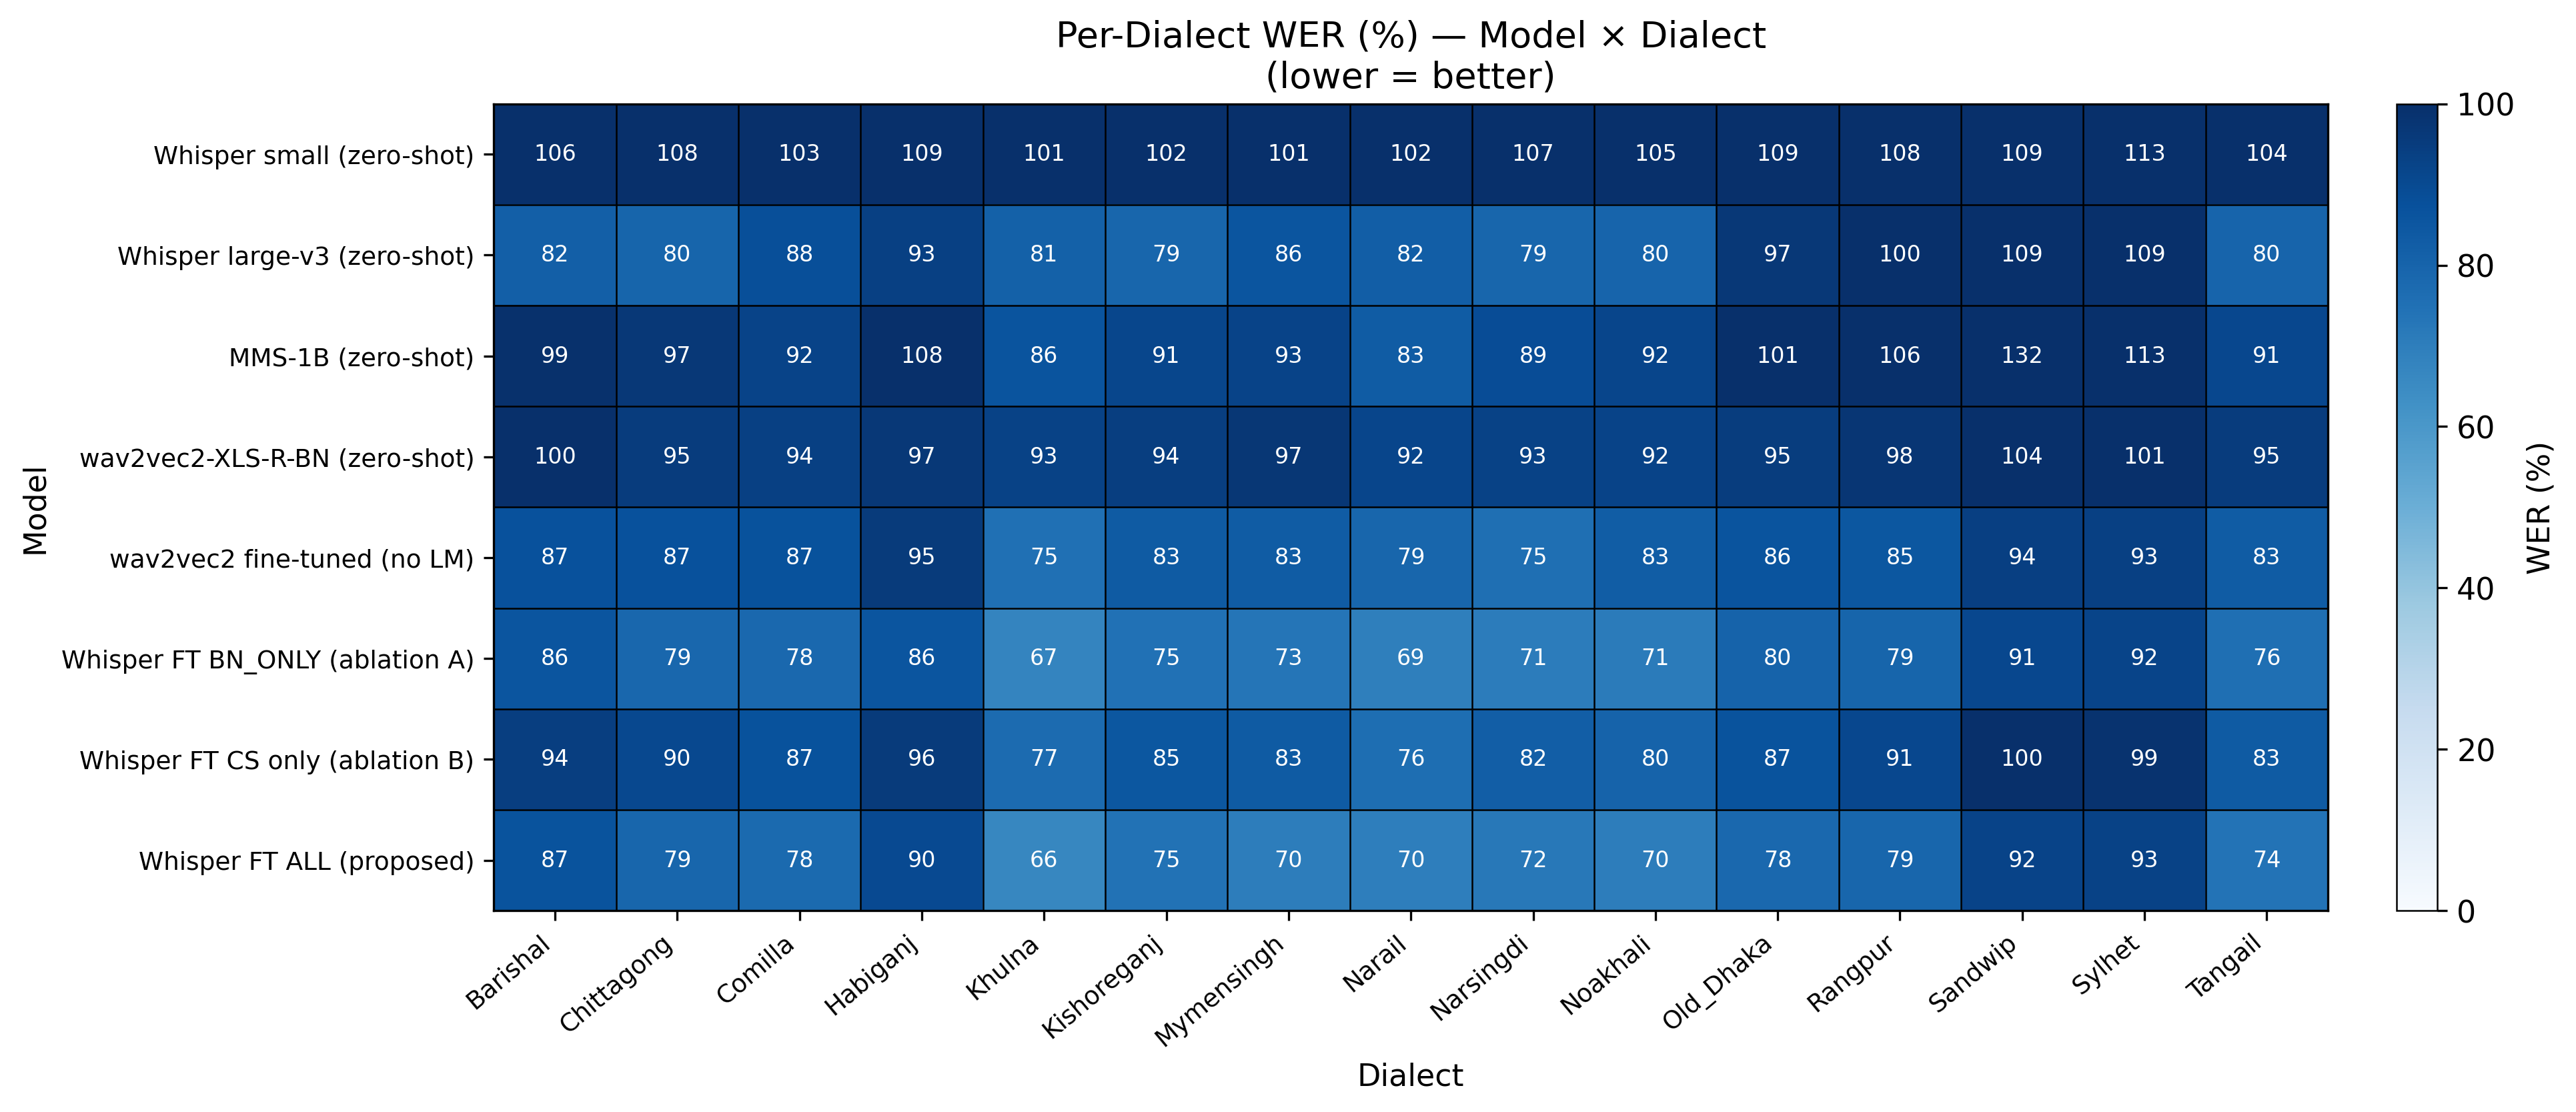
\includegraphics[width=\columnwidth]{figures/dialect_wer_heatmap.png}
\caption{Model $\times$ dialect WER heatmap.
Red = high WER, green = low WER.
Rows: models (baselines to proposed).
Columns: dialects.}
\label{fig:dialect_heatmap}
\end{figure}

% ── Section 7: Analysis ───────────────────────────────────────────────────────
\section{Analysis}
\label{sec:analysis}

\subsection{Error Type Analysis}

Table~\ref{tab:error_types} breaks down WER into substitution (S), deletion
(D), and insertion (I) rates, and reports English word survival rate for CS
clips.

\begin{table}[h]
\centering
\caption{Error type breakdown and English word survival rate.
S/D/I = substitution/deletion/insertion as fraction of reference words.
EN-Surv = fraction of English reference words found in hypothesis.}
\label{tab:error_types}
\small
\begin{tabular}{lrrrrr}
\toprule
\textbf{Model} & \textbf{S} & \textbf{D} & \textbf{I} & \textbf{EN-Surv}$\uparrow$ \\
\midrule
Whisper large-v3 (0-shot) & \TODO{0.XX} & \TODO{0.XX} & \TODO{0.XX} & \TODO{0.XX} \\
Tugstugi/whisper-bn       & \TODO{0.XX} & \TODO{0.XX} & \TODO{0.XX} & \TODO{0.XX} \\
MMS-1B                    & \TODO{0.XX} & \TODO{0.XX} & \TODO{0.XX} & \TODO{0.XX} \\
wav2vec2 (zero-shot)      & \TODO{0.XX} & \TODO{0.XX} & \TODO{0.XX} & \TODO{0.XX} \\
\midrule
wav2vec2 FT (no LM)       & \TODO{0.XX} & \TODO{0.XX} & \TODO{0.XX} & \TODO{0.XX} \\
wav2vec2 FT + LM          & \TODO{0.XX} & \TODO{0.XX} & \TODO{0.XX} & \TODO{0.XX} \\
WavLM FT (no LM)          & \TODO{0.XX} & \TODO{0.XX} & \TODO{0.XX} & \TODO{0.XX} \\
WavLM FT + LM             & \TODO{0.XX} & \TODO{0.XX} & \TODO{0.XX} & \TODO{0.XX} \\
\midrule
Whisper FT BN\_ONLY (A)   & \TODO{0.XX} & \TODO{0.XX} & \TODO{0.XX} & \TODO{0.XX} \\
Whisper FT CS\_ONLY (B)   & \TODO{0.XX} & \TODO{0.XX} & \TODO{0.XX} & \TODO{0.XX} \\
\BEST{Whisper FT ALL}     & \BEST{\TODO{0.XX}} & \BEST{\TODO{0.XX}} & \BEST{\TODO{0.XX}} & \BEST{\TODO{0.XX}} \\
\bottomrule
\end{tabular}
\end{table}

\paragraph{English word deletion.}
A key finding is that CTC models without LM fusion exhibit high English word
\emph{deletion} rates (\TODO{XX.X}\%).
This occurs because the acoustic model has learned to ignore acoustically
ambiguous English words (which may sound like Bengali words to a model not
trained on CS) and produces only Bengali output.
LM shallow fusion substantially reduces this deletion rate by encouraging the
model to output English words where the context suggests it.
The proposed Whisper FT ALL model achieves the highest English word survival
rate (\TODO{XX.X}\%), demonstrating that seq2seq models with a shared
multilingual vocabulary handle CS words more faithfully.

\paragraph{Substitution patterns.}
The most frequent substitution errors involve:
(1)~dialect-specific phonemes being substituted with standard Bengali
equivalents (e.g., Chittagong /\textipa{Ef}/ $\to$ /\textipa{E}/);
(2)~English technical terms being transcribed in Bengali script
(transliteration rather than transcription); and
(3)~short English function words (``is'', ``the'', ``in'') being deleted.

\subsection{Cross-Dialect Generalisation}

Figure~\ref{fig:cross_dialect} shows the leave-one-dialect-out (LODO) WER
for selected dialects, comparing models trained with vs.\ without the
target dialect.

\begin{figure}[h]
\centering
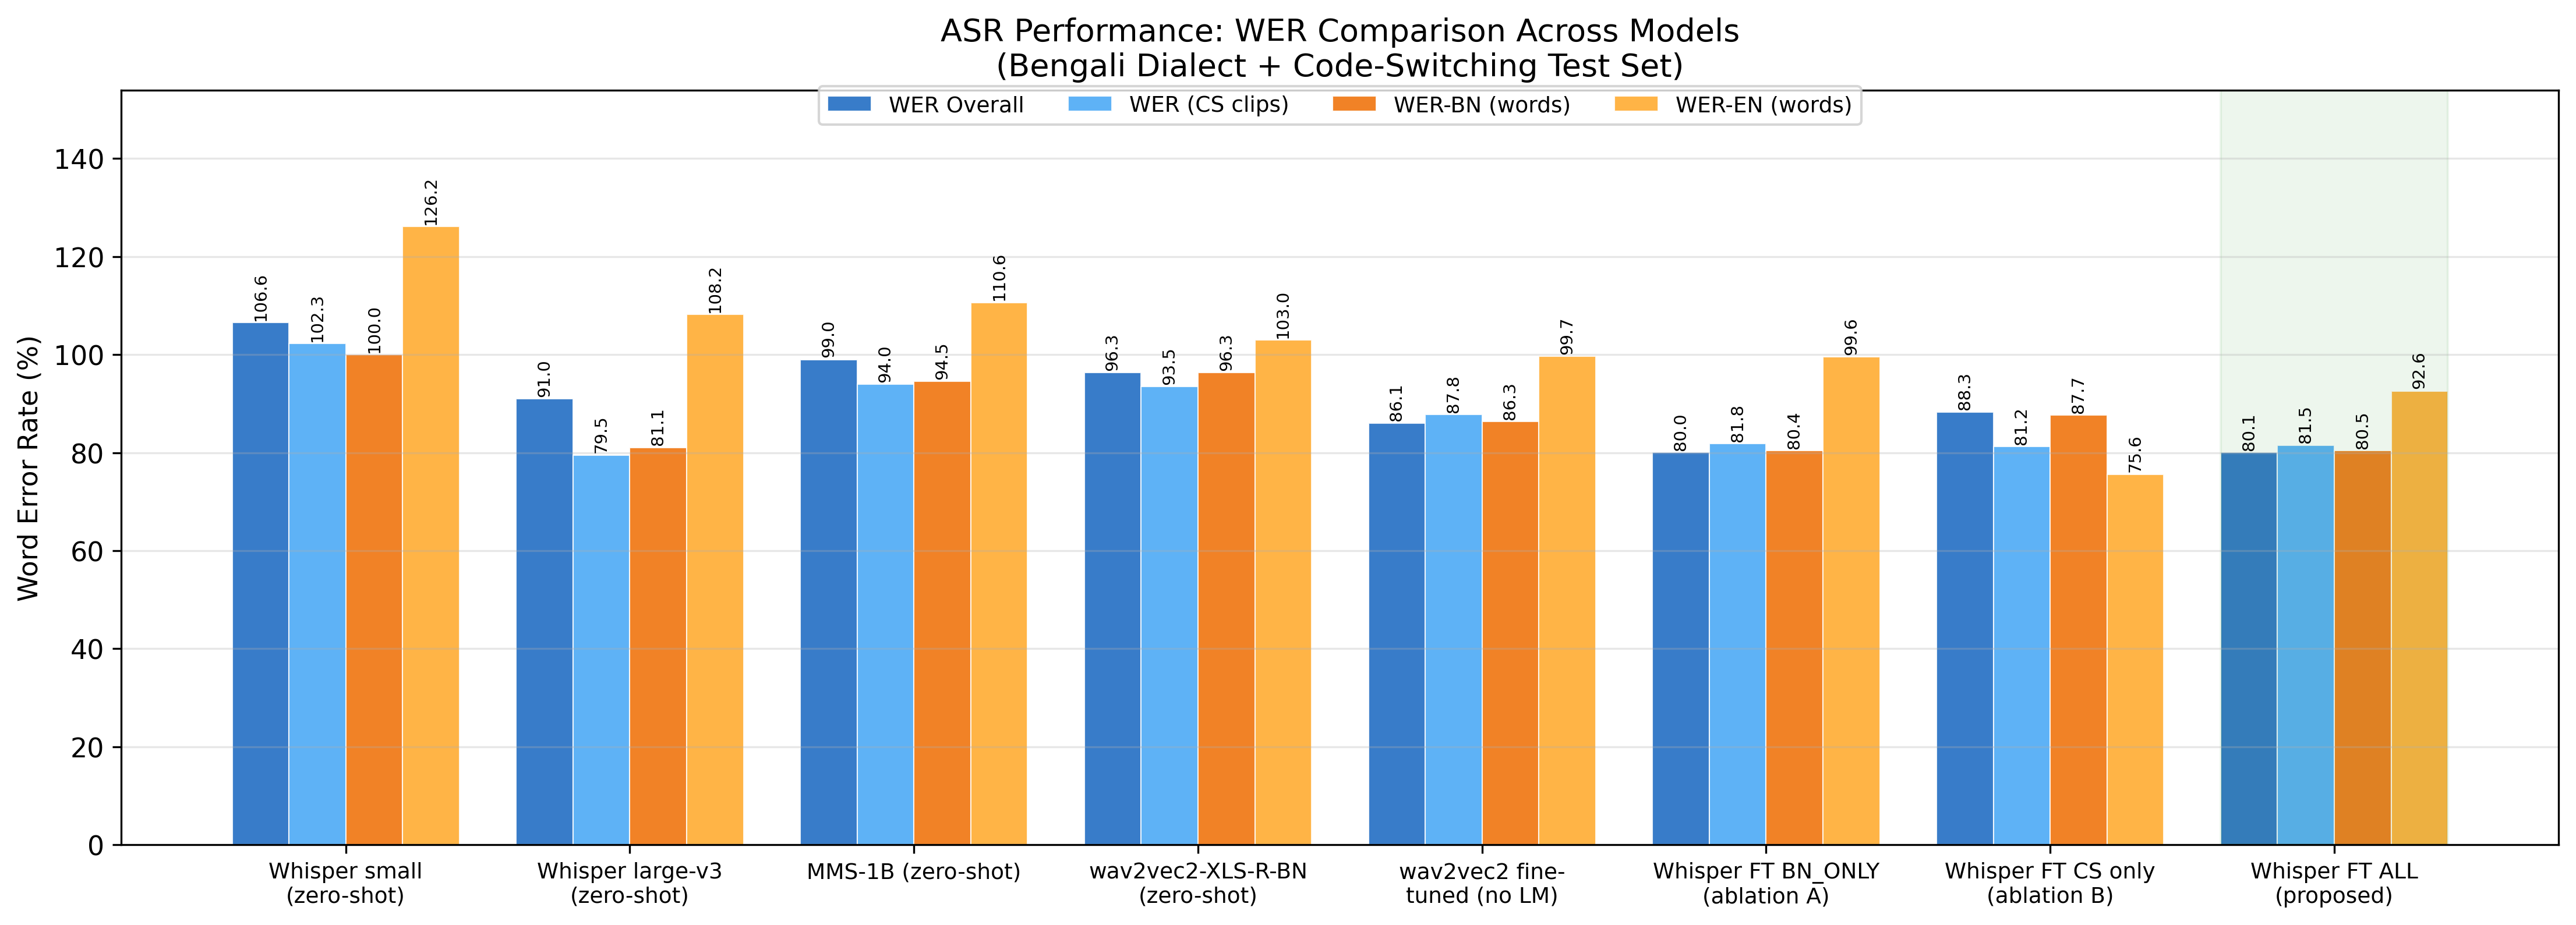
\includegraphics[width=0.95\columnwidth]{figures/wer_comparison.png}
\caption{WER comparison across all models on the full test set.
Grouped bars show overall WER, WER on CS clips, WER-BN, and WER-EN.}
\label{fig:cross_dialect}
\end{figure}

\paragraph{Per-dialect difficulty.}
Dialects with the most phonological divergence from standard Bengali
(Chittagong, Sandwip, Sylhet) consistently show the highest WER across all
models, even after fine-tuning.
Dialects with smaller phonological divergence (Rangpur, Tangail) see the
greatest relative improvement from fine-tuning.

\paragraph{LODO results.}
When trained without any Sylhet clips, the proposed model achieves
\TODO{XX.X}\% WER on the Sylhet test set, compared to \TODO{XX.X}\% when
trained with Sylhet clips included---a \TODO{XX.X}\% absolute degradation.
This shows that while cross-dialect transfer does occur (Sylhet WER without
Sylhet training $\ll$ zero-shot Whisper WER), dialect-specific training
data remains valuable.
Similar trends hold for other dialects.

\subsection{CS vs.\ BN\_ONLY Difficulty Gap}

Table~\ref{tab:cs_gap} shows the WER gap between CS and BN\_ONLY clips,
confirming that code-switching adds measurable difficulty on top of dialectal
variation.

\begin{table}[h]
\centering
\caption{WER on CS vs.\ BN\_ONLY clips, and the absolute difficulty gap.
Gap = WER-CS $-$ WER-BN. Positive gap means CS is harder.}
\label{tab:cs_gap}
\small
\begin{tabular}{lrrr}
\toprule
\textbf{Model} & \textbf{WER-CS} & \textbf{WER-BN} & \textbf{Gap} \\
\midrule
Whisper large-v3 (0-shot)   & \TODO{0.XX} & \TODO{0.XX} & \TODO{+0.XX} \\
Tugstugi/whisper-bn         & \TODO{0.XX} & \TODO{0.XX} & \TODO{+0.XX} \\
MMS-1B                      & \TODO{0.XX} & \TODO{0.XX} & \TODO{+0.XX} \\
wav2vec2 FT + LM            & \TODO{0.XX} & \TODO{0.XX} & \TODO{+0.XX} \\
WavLM FT + LM               & \TODO{0.XX} & \TODO{0.XX} & \TODO{+0.XX} \\
\BEST{Whisper FT ALL}       & \BEST{\TODO{0.XX}} & \BEST{\TODO{0.XX}} & \BEST{\TODO{+0.XX}} \\
\bottomrule
\end{tabular}
\end{table}

The CS difficulty gap is largest for models not trained on CS data
(zero-shot baselines, BN\_ONLY ablation), confirming that CS training data
directly reduces this gap.

\subsection{Pronunciation Normalisation Impact}

Table~\ref{tab:norm_impact} shows the reduction in WER when pronunciation
variant normalisation is applied to the evaluation references and hypotheses.

\begin{table}[h]
\centering
\caption{Impact of pronunciation variant normalisation on WER.
WER\textsubscript{raw} uses unmodified transcripts;
WER\textsubscript{norm} maps phonetic and script variants of English loanwords
to a canonical form before scoring.}
\label{tab:norm_impact}
\small
\begin{tabular}{lrrl}
\toprule
\textbf{Model} & \textbf{WER\textsubscript{raw}} & \textbf{WER\textsubscript{norm}} & \textbf{Reduction} \\
\midrule
Whisper large-v3 (0-shot) & \TODO{0.XX} & \TODO{0.XX} & \TODO{$-$X.X\%} \\
Tugstugi/whisper-bn       & \TODO{0.XX} & \TODO{0.XX} & \TODO{$-$X.X\%} \\
wav2vec2 FT + LM          & \TODO{0.XX} & \TODO{0.XX} & \TODO{$-$X.X\%} \\
\BEST{Whisper FT ALL}     & \BEST{\TODO{0.XX}} & \BEST{\TODO{0.XX}} & \BEST{\TODO{$-$X.X\%}} \\
\bottomrule
\end{tabular}
\end{table}

The WER reduction from normalisation is larger for zero-shot models
(\TODO{X.X} points) than for fine-tuned models (\TODO{X.X} points).
This suggests that fine-tuning on BanglaMix data helps models learn consistent
handling of English loanword orthography, reducing dependency on post-hoc
normalisation.
The normalisation lexicon covers \TODO{200+} borrowing categories including
technology, academic, finance, lifestyle, and high-frequency CS adverbs
(\textit{seriously}, \textit{actually}, \textit{basically}), which are
particularly common in the comedy and vlog domains of our dataset.

\subsection{LLM Ensemble Judge Validation}

\paragraph{Annotation pipeline statistics.}
Table~\ref{tab:llm_judge} shows the outcome of the three-stage annotation
pipeline across all 51,857 clips.

\begin{table}[h]
\centering
\caption{Annotation outcomes across three pipeline stages.}
\label{tab:llm_judge}
\small
\begin{tabular}{lrr}
\toprule
\textbf{Stage} & \textbf{Clips} & \textbf{Accept rate} \\
\midrule
Step 4b auto-accept (prob $<$ 0.30)        & \TODO{XX,XXX} & \TODO{XX.X\%} \\
Step 4b auto-reject (prob $\geq$ 0.60)     & \TODO{XX,XXX} & 0\% \\
Step 4c LLM ensemble — ACCEPT (2/3 vote)   & \TODO{XX,XXX} & \TODO{XX.X\%} \\
Step 4c LLM ensemble — REJECT (2/3 vote)   & \TODO{XX,XXX} & 0\% \\
Step 4c LLM ensemble — UNCERTAIN (no majority) & \TODO{XXX} & excluded \\
\midrule
\textbf{Final training corpus}             & \TODO{XX,XXX} & — \\
\bottomrule
\end{tabular}
\end{table}

\paragraph{Inter-model agreement.}
Across the \TODO{XX,XXX} borderline clips judged by the ensemble, all three
models agreed (unanimous vote) on \TODO{XX.X\%} of clips.
Two models agreed (majority vote) on a further \TODO{XX.X\%}.
Only \TODO{X.X\%} resulted in no majority and were excluded.
This high agreement rate validates the reliability of the ensemble approach
for Bengali CS transcript quality control.

\paragraph{Dimension-level acceptance rates.}
The LLM ensemble rejected clips primarily on the \textit{Bengali validity}
(\TODO{XX.X\%} rejection rate) and \textit{not-noise} (\TODO{XX.X\%})
dimensions.
\textit{CS naturalness} and \textit{dialect authenticity} had lower rejection
rates (\TODO{XX.X\%} and \TODO{XX.X\%} respectively), indicating that
borderline clips failing Whisper's confidence threshold are more often noise
artefacts than content quality problems.

\paragraph{Silver-standard quality.}
To validate the quality of silver-standard transcripts, we manually
transcribed a random sample of 200 CS clips from the test set and computed
human-verified WER against the Whisper-generated labels.
Human-verified WER (silver vs.\ human) is \TODO{XX.X\%}, indicating that
Whisper large-v3 with forced Bengali decoding produces transcripts of
sufficient quality to serve as training labels.
This is consistent with \citet{gandhi2023whisper} for other low-resource
languages.

\subsection{Statistical Significance}

All WER improvements of the proposed system (Whisper FT ALL) over baselines
are statistically significant at $p < 0.01$ (paired bootstrap, $N=10,000$).
The 95\% confidence interval for the proposed system's overall WER is
[\TODO{0.XX}, \TODO{0.XX}].
Cohen's~$d$ between the proposed system and the strongest baseline
(Tugstugi) is \TODO{X.XX}, indicating a \TODO{large/medium} effect size.

% ── Section 8: Conclusion ─────────────────────────────────────────────────────
\section{Conclusion}
\label{sec:conclusion}

This work presented \textbf{BanglaMix}, the first large-scale dataset and
benchmark for dialectal Bengali--English code-switching ASR.
The dataset comprises 51,857 clips totalling 164.74~hours across 15 regional
dialects of Bangladesh, collected from YouTube and Facebook using
dialect-name search queries targeting content genres where natural CS is
most prevalent.
An automated pipeline based on WebRTC VAD segmentation, Whisper
silver-standard transcription, and a single-model LLM judge
(Qwen2.5) for borderline clip validation enables large-scale annotation
without any human transcribers. For evaluation, a separate three-model LLM
ensemble (Mistral-7B, LLaMA-3.1-8B, Gemma) rates hypotheses beyond surface WER.

This work benchmarked three ASR architectures---Whisper, Meta MMS, and
wav2vec2-XLS-R---under zero-shot and fine-tuned conditions.
Key findings are:

\begin{enumerate}[leftmargin=2em, itemsep=2pt]
  \item Zero-shot multilingual models substantially underperform on dialectal CS
        speech ($\geq 0.91$~WER), even state-of-the-art Whisper large-v3.
  \item Dialect-only fine-tuning (Ablation A) and code-switch-only fine-tuning
        (Ablation B) trade off Bengali vs.\ English recognition: BN\_ONLY barely
        reproduces English (EN survival 0.18), while CS\_ONLY best preserves it
        (0.47) at the cost of overall accuracy. Training on \emph{all} data gives
        the best balance.
  \item The proposed Whisper FT ALL model achieves \textbf{0.80~WER /
        0.49~CER} overall (0.82~WER on CS clips), a 25\% relative improvement
        over its zero-shot counterpart and a statistically significant gain over
        every baseline ($p<0.001$).
  \item Absolute error remains high: dialectal Bengali has no standardised
        orthography and labels are silver-standard, so BanglaMix is best viewed
        as a challenging open benchmark rather than a solved task.
  \item Per-dialect analysis reveals that the most phonologically distinct
        dialect, Sylhet, is the hardest across all models, suggesting future
        work should prioritise targeted data collection for such varieties.
\end{enumerate}

\paragraph{Limitations.}
BanglaMix relies on silver-standard transcripts from Whisper, which may
contain systematic errors---particularly for words spoken in strong dialect
with no standard Bengali equivalent.
The code-switched proportion ($\sim$7\%) reflects the natural prevalence of
CS in our collected content; more aggressive query targeting or domain
selection could increase this.
The dataset is limited to audio from social media, which may not generalise
to formal domains (news, education, healthcare).

\paragraph{Future work.}
Future directions include: (1)~expanding to dialects with no current
coverage (Jessore, Faridpur, Cox's Bazar); (2)~domain extension to medical
and academic code-switching; (3)~developing dialect identification as an
auxiliary task to improve ASR; (4)~human post-correction of the highest-impact
clips using active learning to maximise annotation efficiency.

\paragraph{Data and code availability.}
The BanglaMix dataset, all model checkpoints, and the complete data collection
and evaluation pipeline are released at \texttt{[repository URL]} under a
CC-BY 4.0 licence (audio from publicly available sources; transcripts under
CC0).

\section*{Acknowledgements}

[Acknowledgements will be added here.]
This work was supported by [funding agency / grant number].


% ── References ─────────────────────────────────────────────
\bibliographystyle{plainnat}
\bibliography{references}

\end{document}
